\section{Durchführung}
\label{sec:Durchführung}
Der in diesem Versuch verwendete Aufbau ist in \autoref{fig:Aufbau} dargestellt.
\begin{figure}[H]
    \centering
    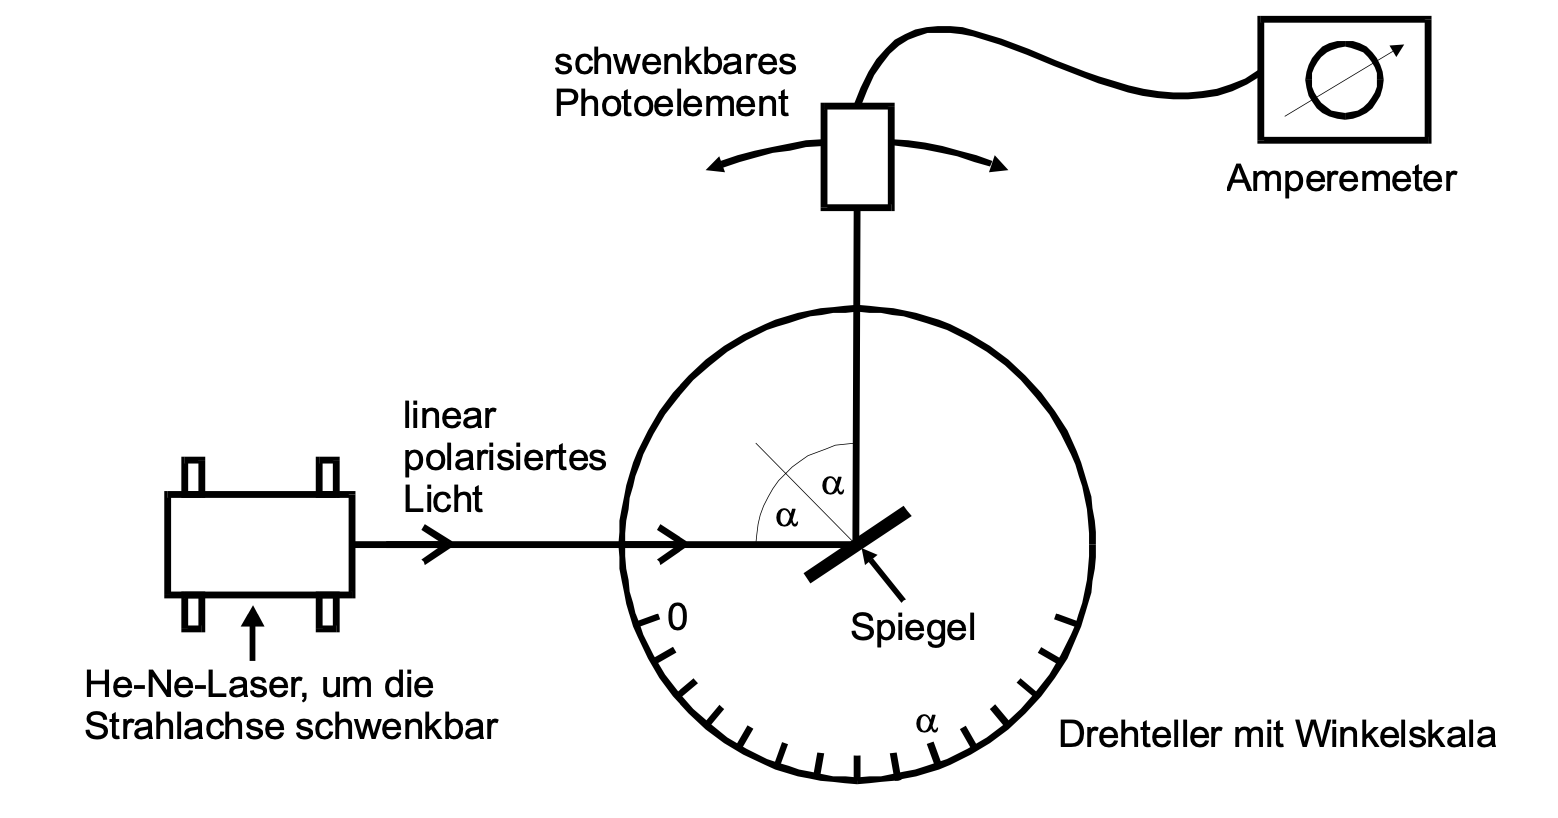
\includegraphics[height=6cm]{content/pics/Aufbau.png}
    \caption{Schematischer Aufbau des Experimentes \cite{v407}.}
    \label{fig:Aufbau}
\end{figure}
Der verwendete Laser emmittiert kein polarisiertes Licht, weswegen zwischen Laser und
Spiegel ein Polarisationsfilter gesetzt wird. Der drehbare Spiegel ist im Detail in 
\autoref{fig:Spiegel} gezeigt.
\begin{figure}[H]
    \centering
    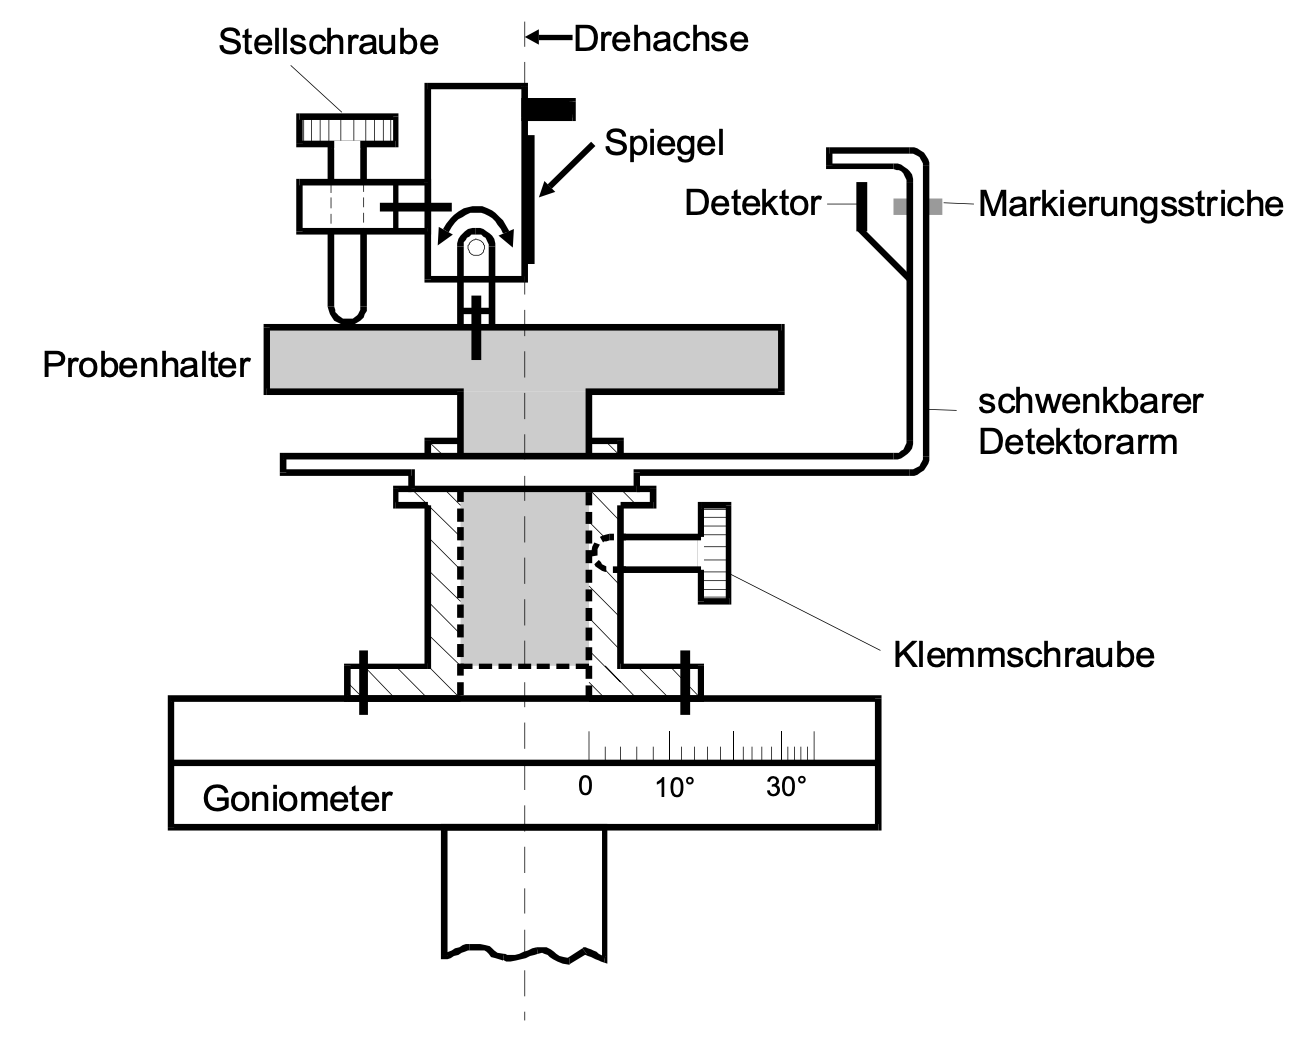
\includegraphics[height=6cm]{content/pics/Goniometer.png}
    \caption{Skizze des verwendeten drehbaren Spiegels mit Goniometer \cite{v407}.}
    \label{fig:Spiegel}
\end{figure}

Bevor die eigentliche Messung starten kann, werden eine Null- und eine Dunkelmessung durchgeführt.
Für die Dunkelmessung wird der Photostrom ohne eingeschalteten Laser mithilfe der Photozelle gemessen, wohingegen bei
der Nullmessung der Laser eingeschaltet wird.

In einem nächsten Schritt wird der Spiegel in die Apparatur eingesetzt und so ausgerichtet, dass ein Winkel von
$\alpha = \qty{0}{\degree}$ gemessen wird, wenn der Laser zurück in die Öffnung strahlt.

Nach der Kalibrierung werden die Photoströme für Winkel zwischen $\qty{5}{\degree}$ und $\qty{87}{\degree}$ gemessen,
wobei alle $\qty{2}{\degree}$ ein Wert für s-polarisiertes und ein Wert für p-polarisiertes Licht aufgenommen wird.
